%% Version 2022-07-08
%% LaTeX-Vorlage für Abschlussarbeiten
%% Erstellt von Nils Potthoff, ab 2020 erneuert und ausgebaut von Simon Lohmann
%% Lehrstuhl Automatisierungstechnik/Informatik Bergische Universität Wuppertal
%%%%%%%%%%%%%%%%%%%%%%%%%%%%%%%%%%%%%%%%%%%%%%%%%%%%%%%%%%%%%%%%%%%%%%%%%%%%%%%%

\chapter{Anhang}
	\label{sec:anhang}
	
	%\section{Gebäudebestand in Deutschland: Wohnflächen-Häufigkeit nach Basis-Typen / Baujahr}
		%\autoref{tab:Gebäudematrix_2011} zeigt \autoref{sec:Grundlagen:Wärmewende_in_D:Ausgangssituation} 
		
		\begin{table}[!h]
			\includegraphics[width=\textwidth]{Medien/own/IWU_2015_S18_Gebäudestandsmatrix_Stand_2011_Diefenbach_2013.png}
			\caption{Gebäudematrix mit Gebäudetypologiesierung aus den Daten des Zensus 2011 ohne Gebäudetypen Hochhaus(HH) und Sonderfälle(F/F, NBL\_x) Erläuterung der Kürzel: EFH \= Einfamilienhaus, RH \= Reihenhaus, MFH = Mehrfamilienhaus, GMH \= großes Mehrfamilienhaus \cite[S.~18]{IWU_2015_Wohngebäudetypologie}}
			\label{tab:Gebäudematrix_2011}
		\end{table}	
		\todo{Quelle}
			
%		\begin{figure}[!h]
%			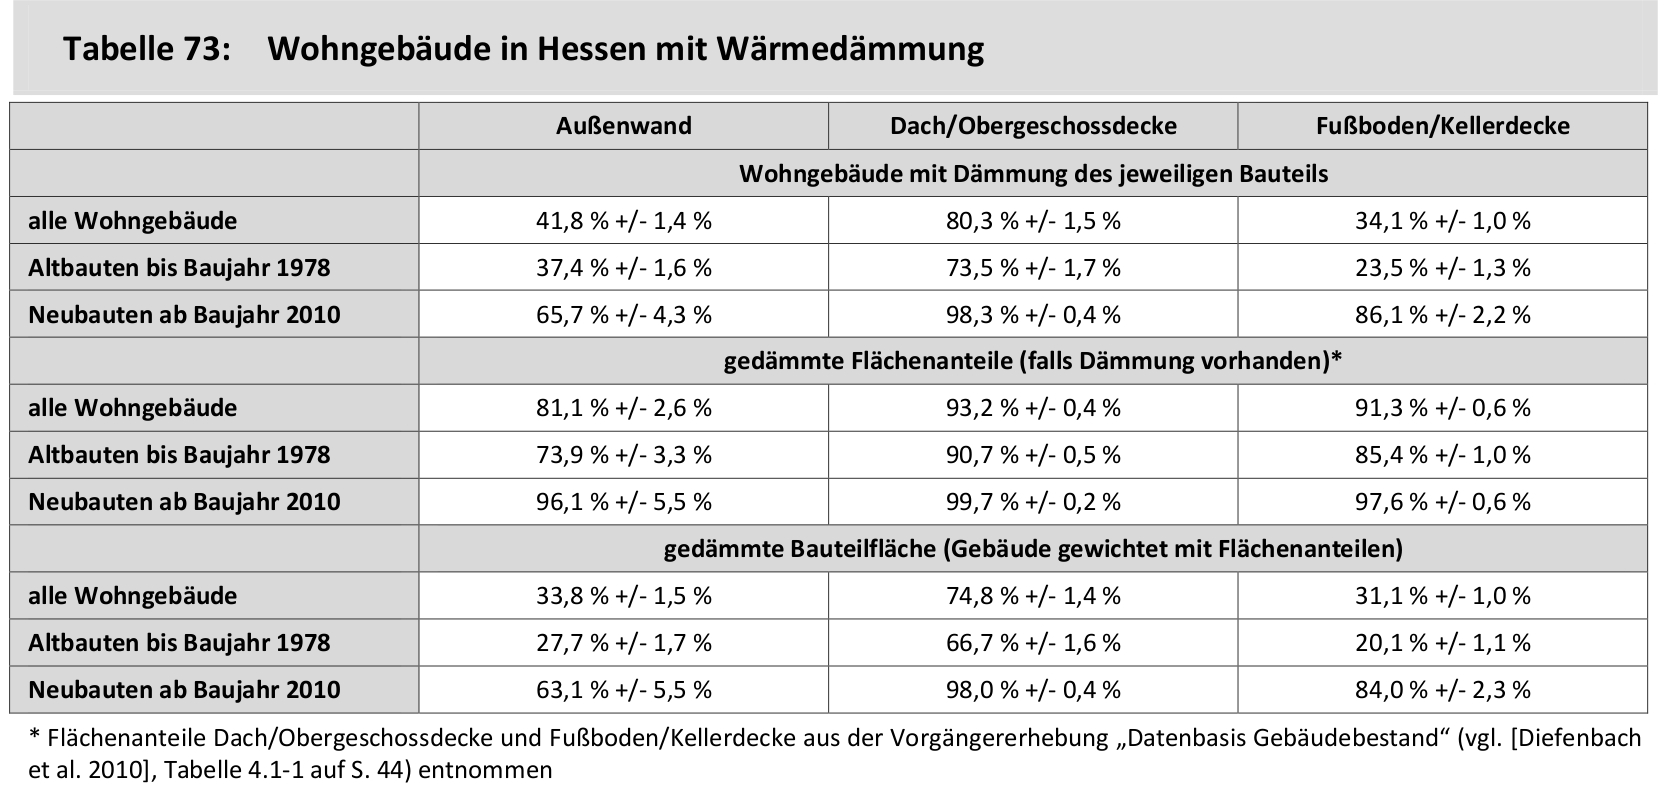
\includegraphics[width=\textwidth]{Medien/own/IWU_2018_Gebaeude_in_Hessen_mit_Waermedaemmung_S_108.png}
%			\caption{Wohngebäude in Hessen mit Wärmedämmung, Stand 2018 [IWU 2018]}
%			\label{tab:Gebäude_Hessen_Dämmung_2018_orig}
%		\end{figure}
%		\todo{Quelle}
					
%		\begin{figure}[!h]
%			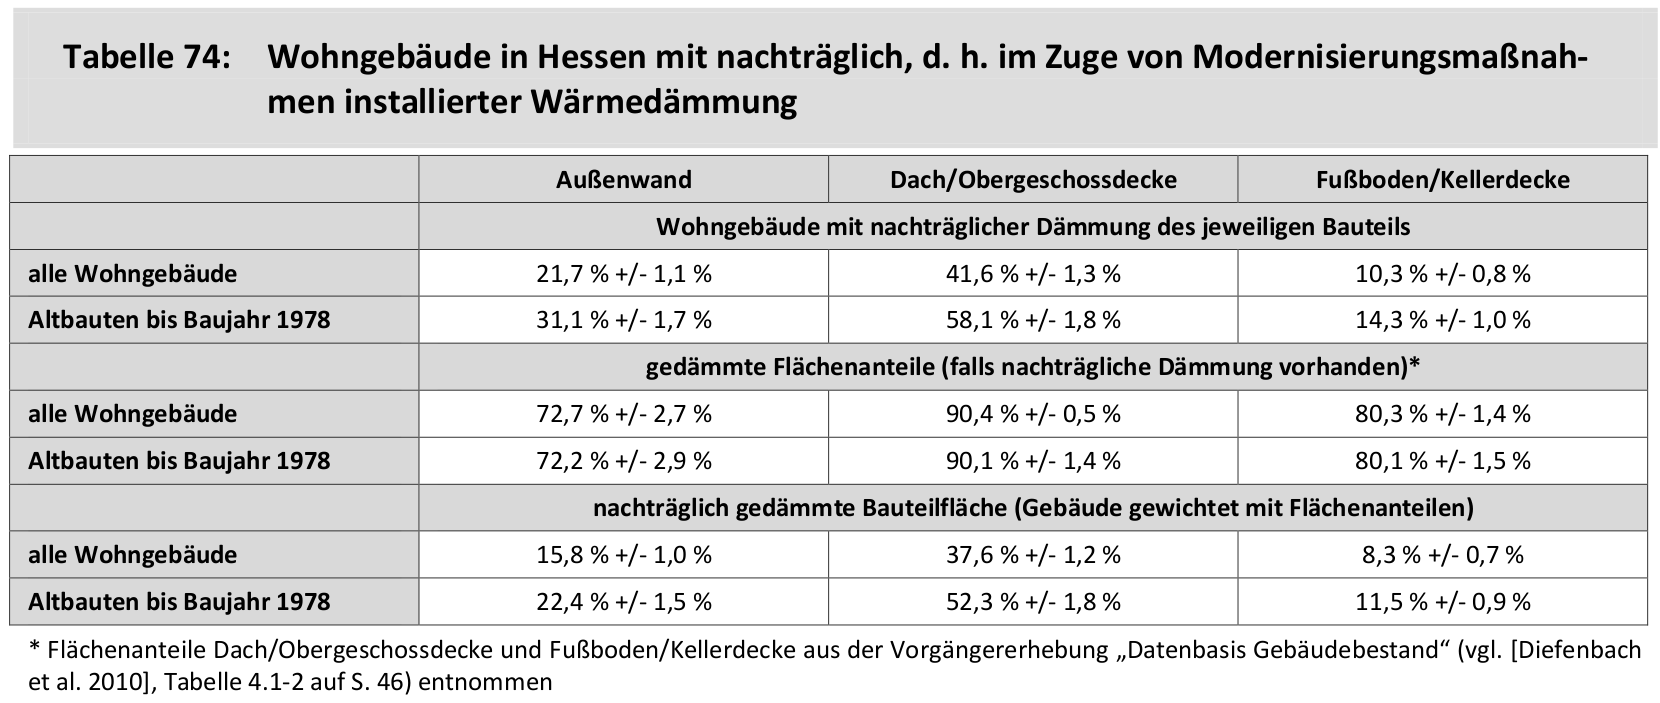
\includegraphics[width=\textwidth]{Medien/own/IWU_2018_Gebaeude_in_Hessen_mit_nachtraeglicher_Waermedaemmung_S_108.png}
%			\caption{Wohngebäude in Hessen mit nachträglicher Wärmedämmung, Stand 2018 [IWU 2018]}
%			\label{tab:Gebäude_Hessen_Dämmung_nachträglich_2018_orig}
%		\end{figure}
%		\todo{Quelle}
		
	%\section{Vojens Versorgungsgebiet (Dänemark)}
	%	\autoref{fig:Vojens_Fernwärmenetz_Plan} zeigt den Netzplan des Versorgungsgebietes des in \autoref{sec:Grundlagen:Wärmewende_in_D:Beispiel_Wärmeplan_Fernwärmenetz} beschriebenen Fernwärmenetzes Vojens in Dänemark.
		
		\begin{figure}[!h]
			\includegraphics[width=1.00\linewidth]{Medien/own/Vojens_Fernwärme_Netzplan.png}
			\caption{Fernwärmenetz Vojen, Netzausbau (lila), Stand 2006 \cite{web_vojens_plan}}
			\label{fig:Vojens_Fernwärmenetz_Plan}
		\end{figure}
	
	\begin{figure}[h]
		\centering
		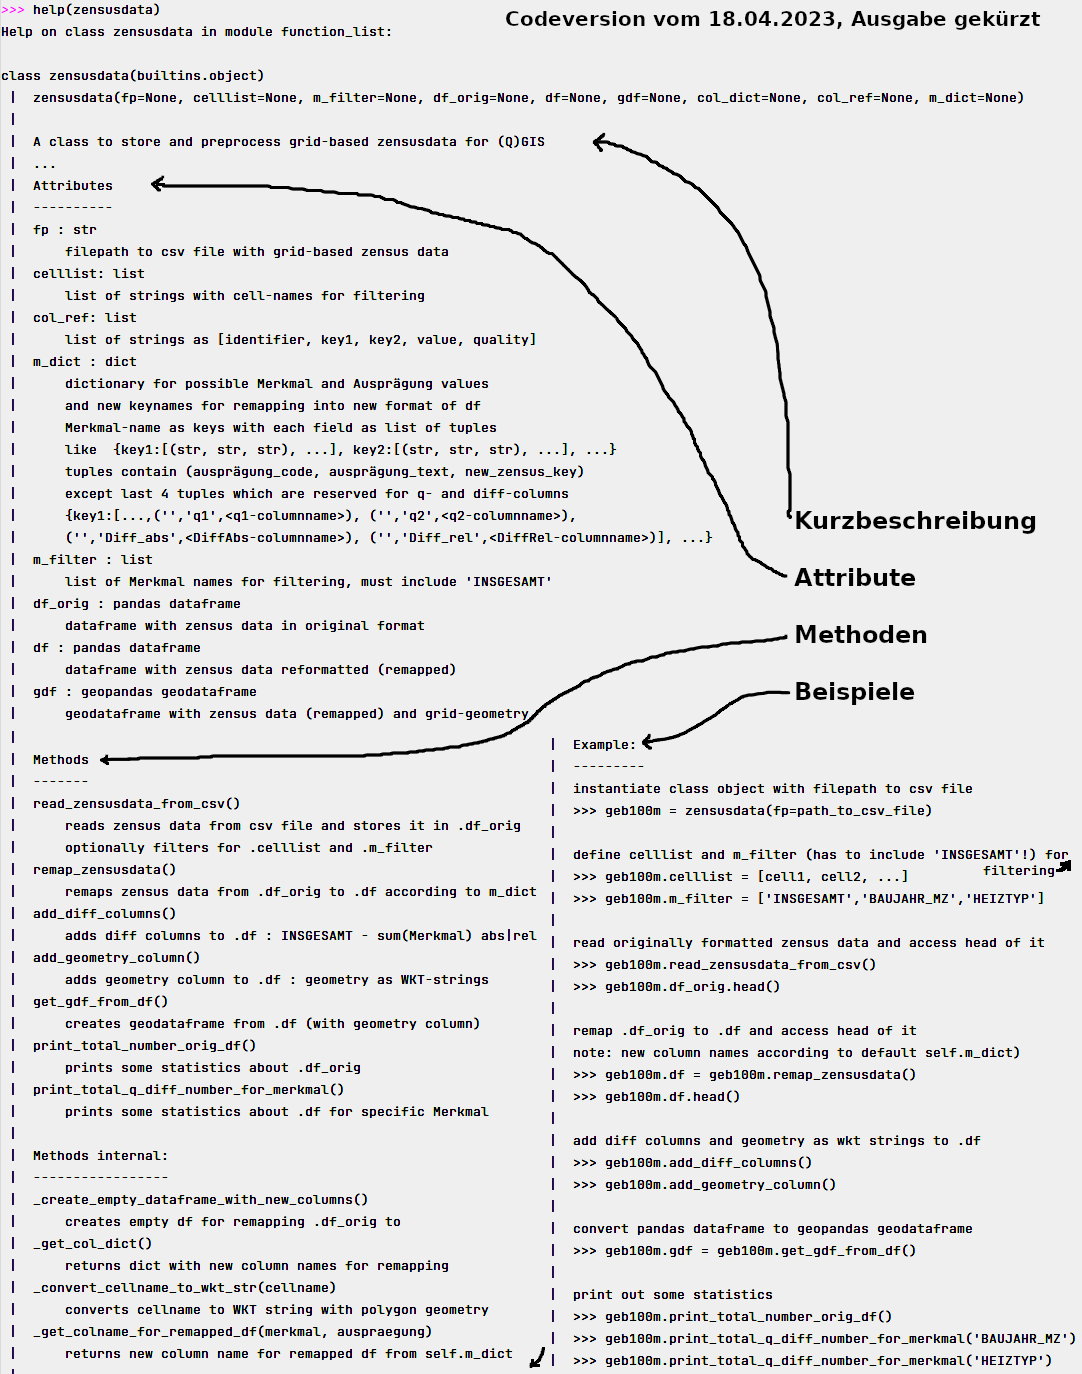
\includegraphics[width=\linewidth]{./Medien/own/help_zensusdata2.png}
		\caption{Ausgabe des Docstrings der Klasse \textit{zensusdata}}
		\label{fig:help_zensusdata}
	\end{figure}

	\begin{figure}[h]
		\centering
		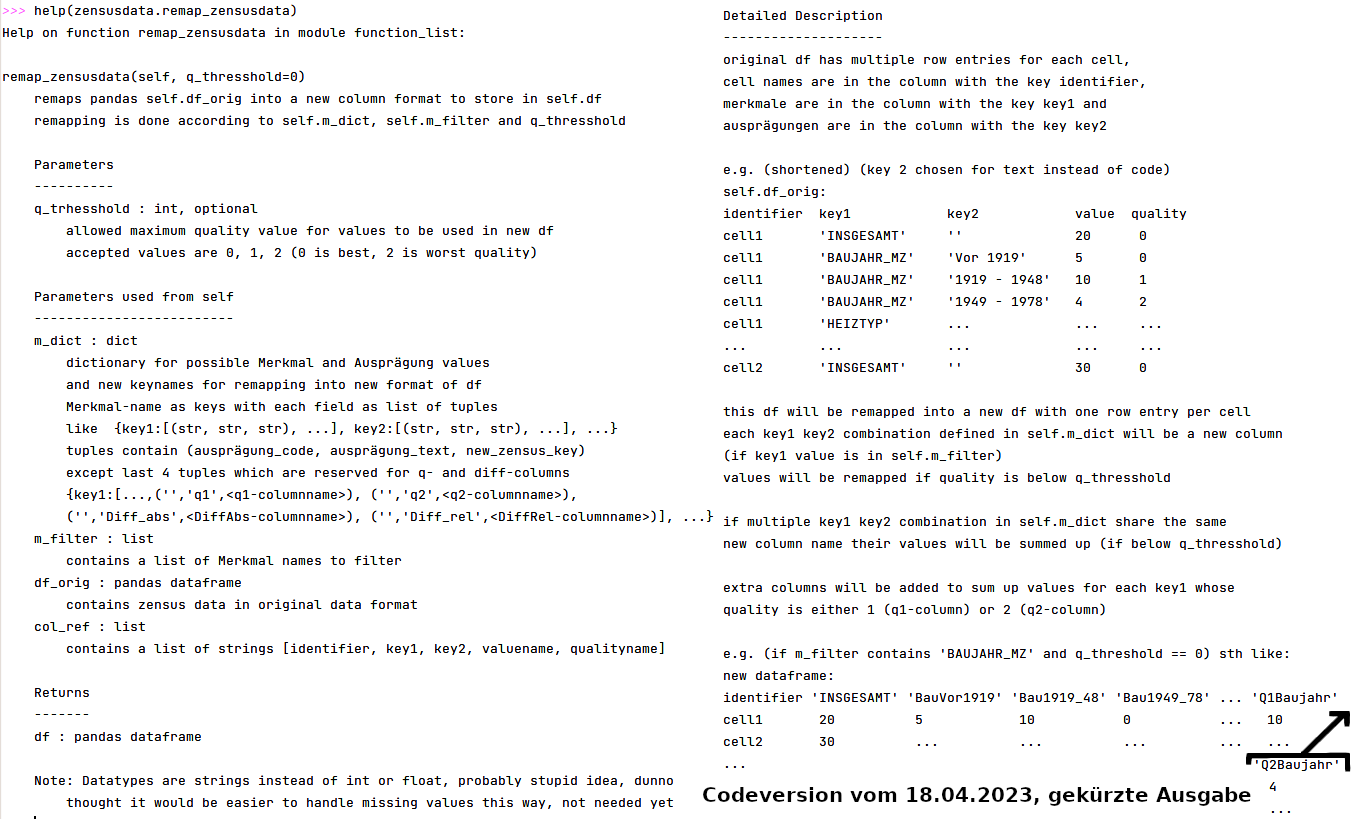
\includegraphics[angle=90,width=0.8\linewidth]{./Medien/own/help_zensusdata.remap_zensusdata.png}
		\caption{Ausgabe des Docstrings der Methode \textit{remap\_zensusdata()} der Klasse \textit{zensusdata}}
		\label{fig:help_zensusdata.remap_zensusdata}
	\end{figure}

	
	\begin{table}[h]
		\centering
		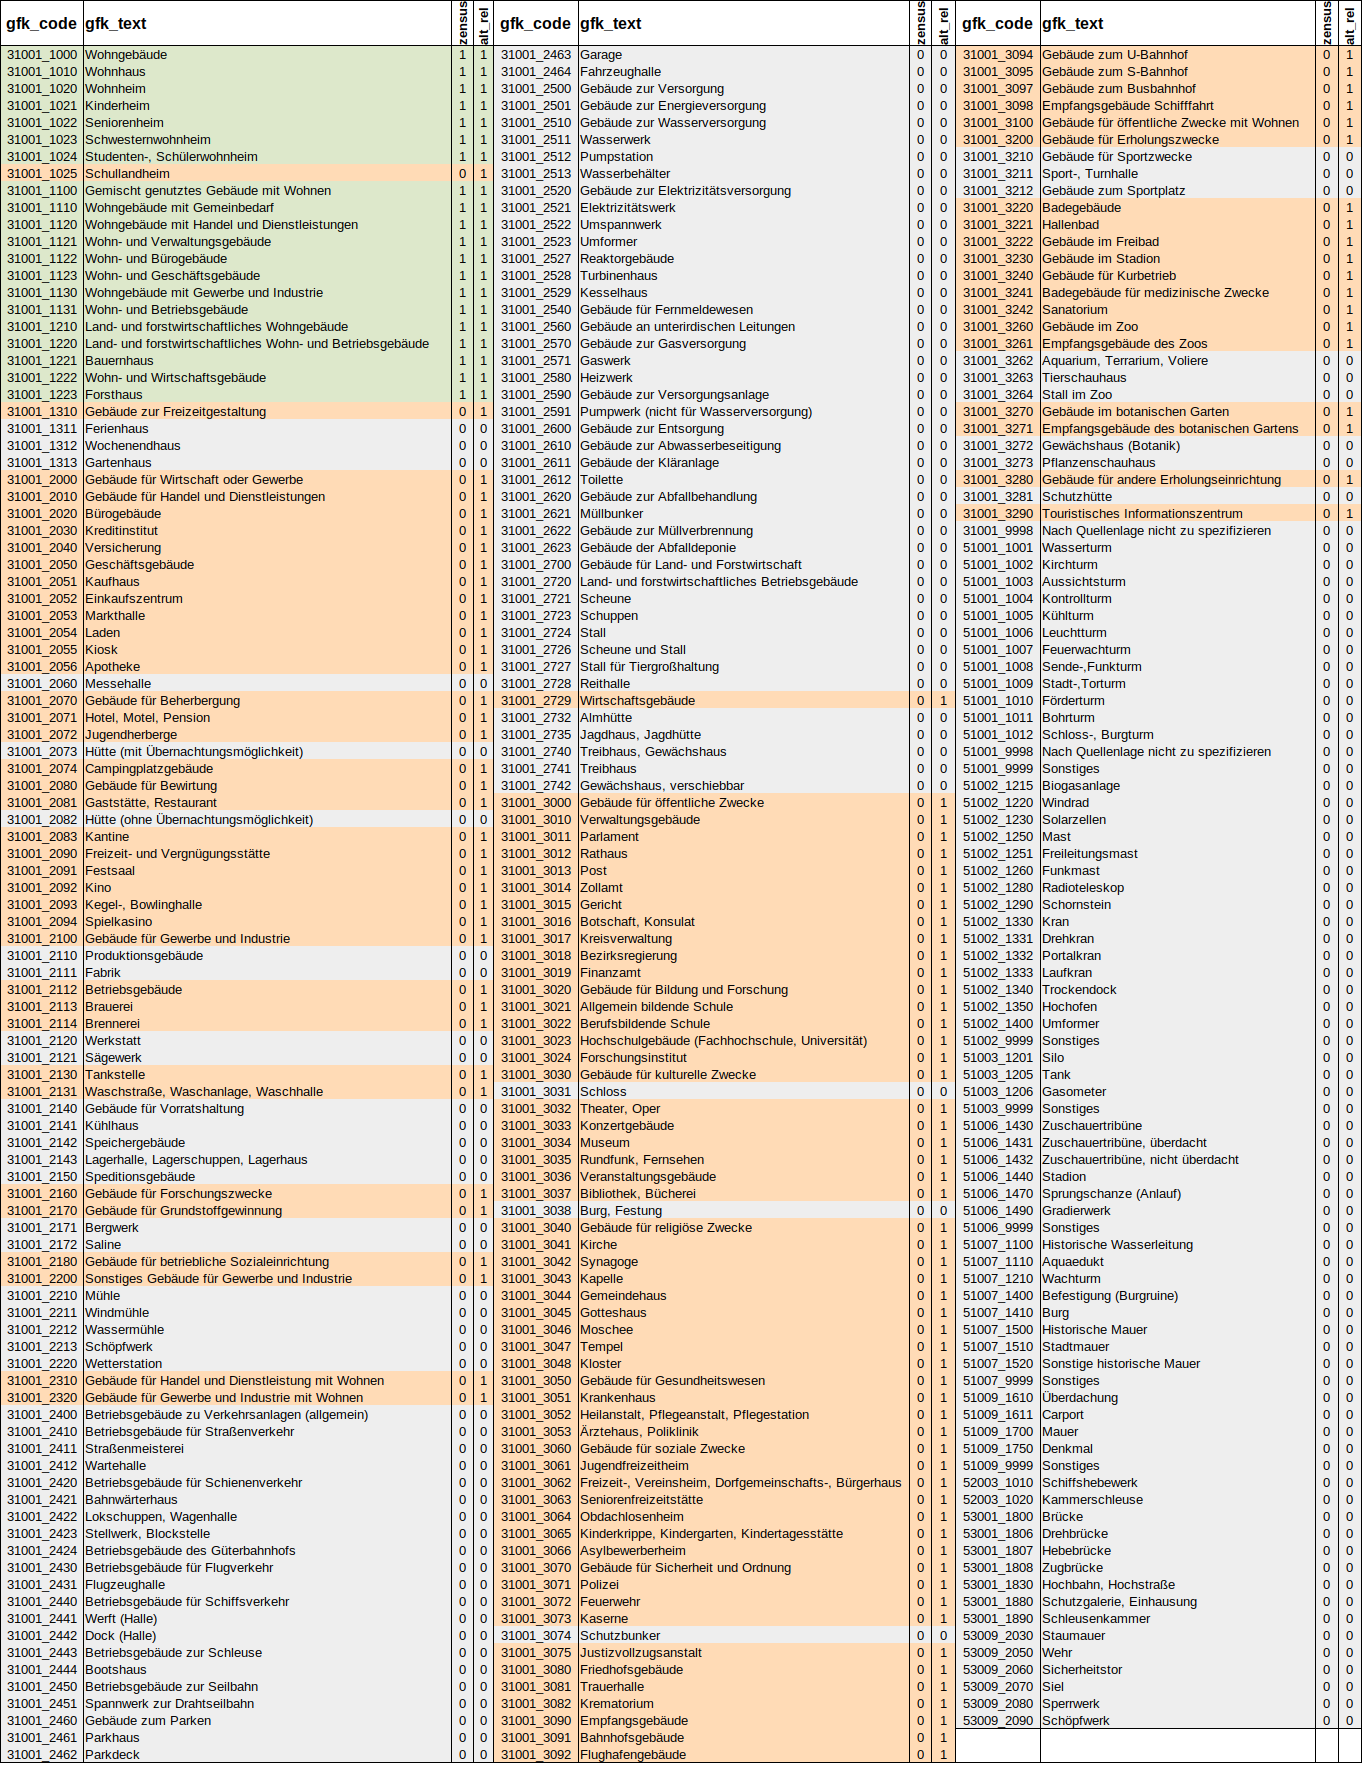
\includegraphics[width=\linewidth]{./Medien/tables/gfk_codes_texts_flags_all.png}
		\caption{Liste aller ALKIS (und ATKIS) GFK-Codes und -Texten inkl. selbst gesetzter Flags \cite{web_download_alkis_gebaeudefunktion_code_definition}\cite{web_github_repo_code}}
		\label{tab:gfk_codes_texte_flags_all}
	\end{table}
	
		
	
	%\section{Hausumringe Geometrien-Vergleich [ALKIS, LANUV, OSM]}
	
		\begin{figure}[h]
			\centering
			\subfloat[Subfigure 1 list of figures text][Amtliche Basiskarte (ABK)]{
				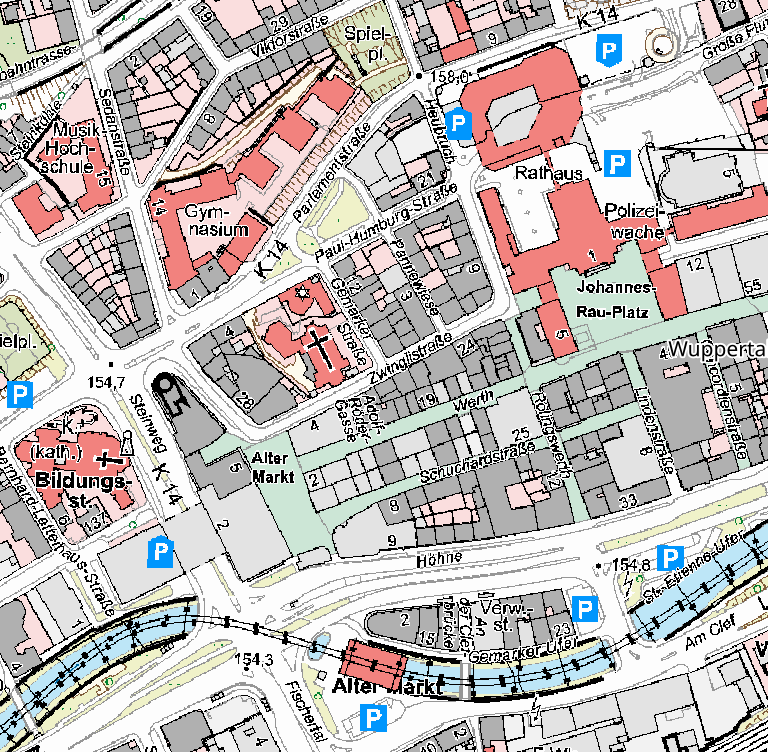
\includegraphics[width=0.3\textwidth]{Medien/own/hu_vergleich/qgis_hu_vergleich_abk.png}
				\label{fig:analyse:hu_vergleich_detail_01}}
			\subfloat[Subfigure 2 list of figures text][ALKIS + LANUV + OSM]{
				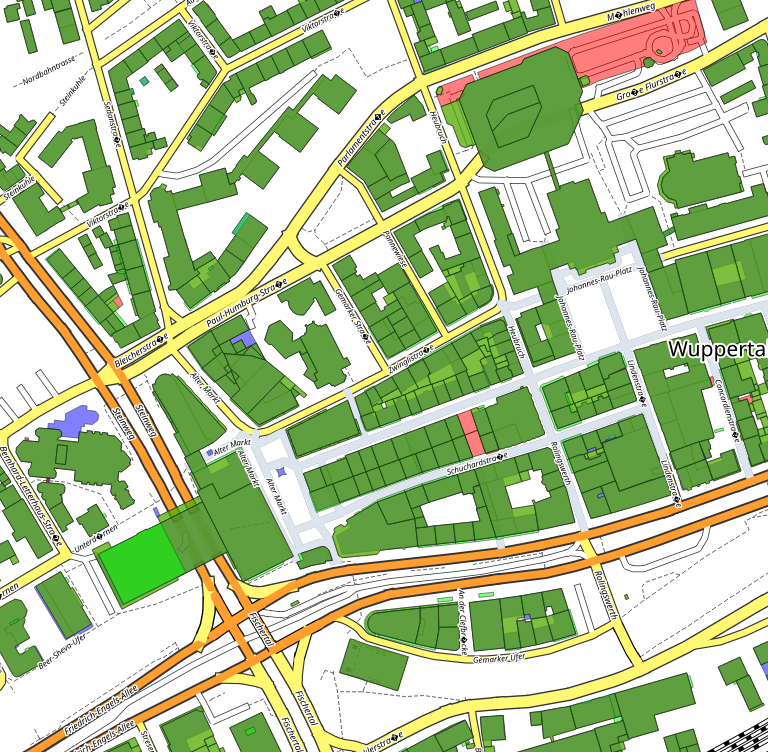
\includegraphics[width=0.3\textwidth]{Medien/own/hu_vergleich/qgis_hu_vergleich_alkis_lanuv_osm.png}
				\label{fig:analyse:hu_vergleich_detail_02}}
			\subfloat[Subfigure 3 list of figures text][Legende Hausumringe]{
				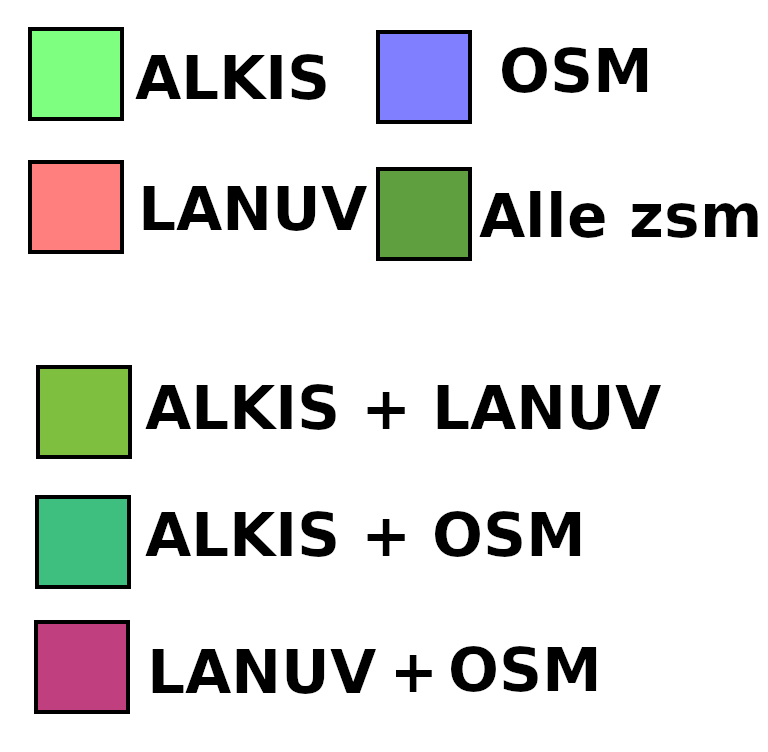
\includegraphics[width=0.3\textwidth]{Medien/own/hu_vergleich/qgis_hu_vergleich_legende2.png}
				\label{fig:analyse:hu_vergleich_detail_03}}
			\qquad
			\subfloat[Subfigure 4 list of figures text][Hausumringe ALKIS]{
				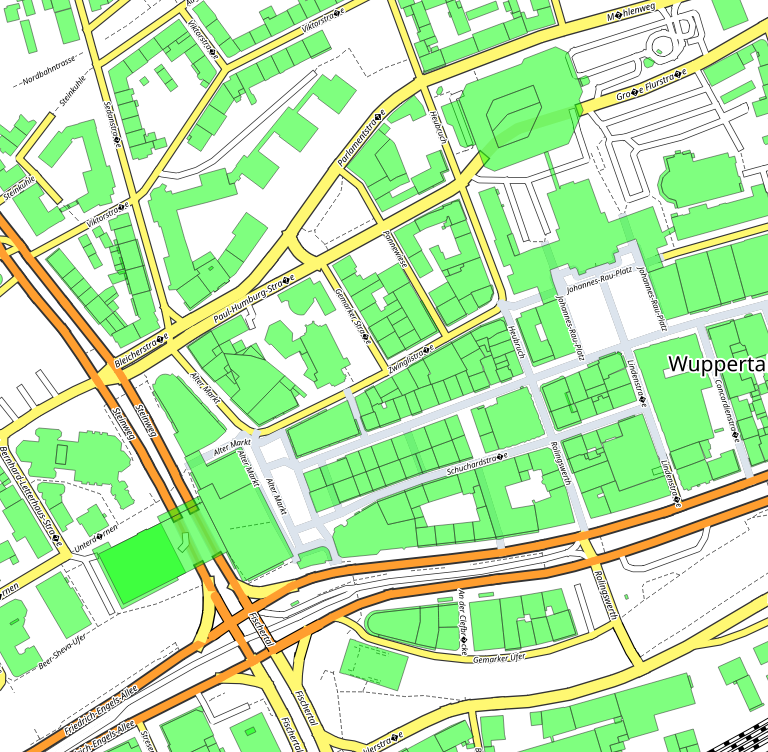
\includegraphics[width=0.3\textwidth]{Medien/own/hu_vergleich/qgis_hu_vergleich_alkis.png}
				\label{fig:analyse:hu_vergleich_detail_04}}
			\subfloat[Subfigure 5 list of figures text][Hausumringe LANUV]{
				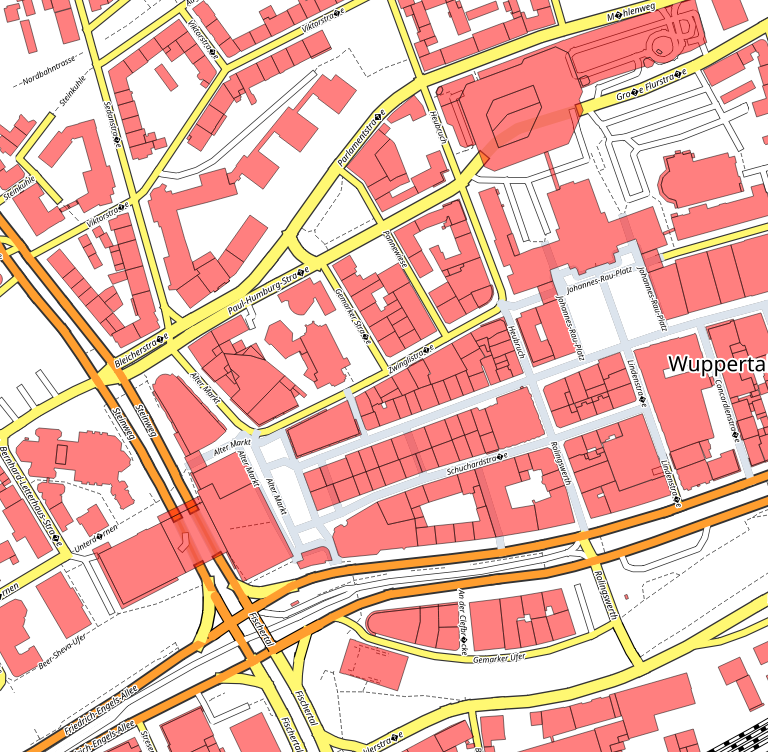
\includegraphics[width=0.3\textwidth]{Medien/own/hu_vergleich/qgis_hu_vergleich_lanuv.png}
				\label{fig:analyse:hu_vergleich_detail_05}}
			\subfloat[Subfigure 6 list of figures text][Hausumringe OSM]{
				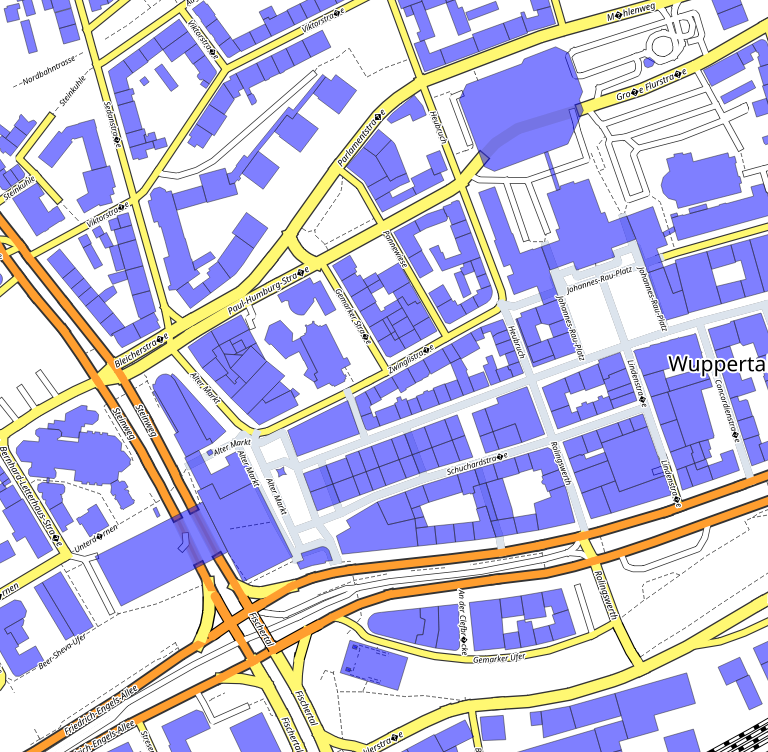
\includegraphics[width=0.3\textwidth]{Medien/own/hu_vergleich/qgis_hu_vergleich_osm.png}
				\label{fig:analyse:hu_vergleich_detail_06}}
			\qquad
			\subfloat[Subfigure 7 list of figures text][ABK + ALKIS]{
				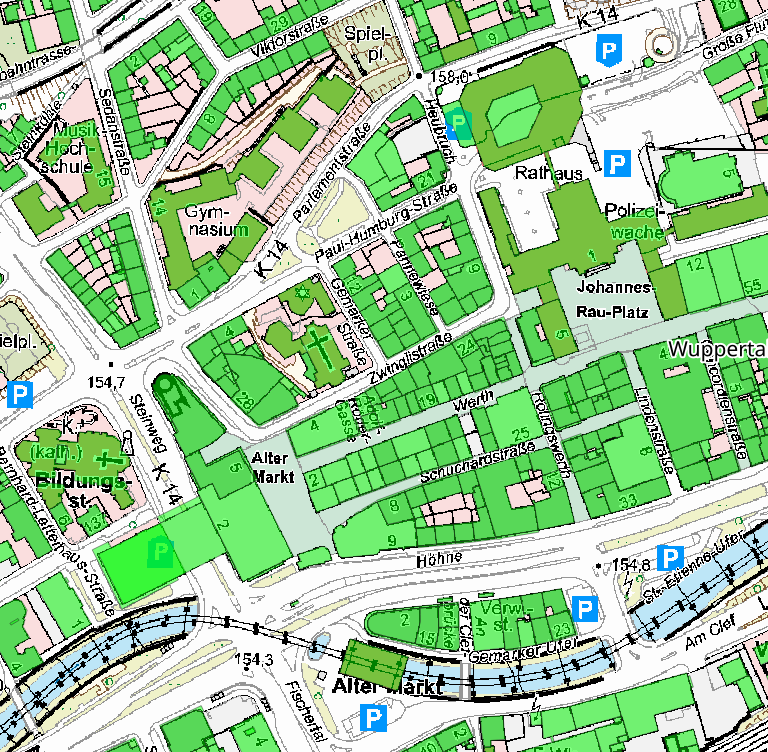
\includegraphics[width=0.3\textwidth]{Medien/own/hu_vergleich/qgis_hu_vergleich_abk_alkis.png}
				\label{fig:analyse:hu_vergleich_detail_07}}
			\subfloat[Subfigure 8 list of figures text][ABK + LANUV]{
				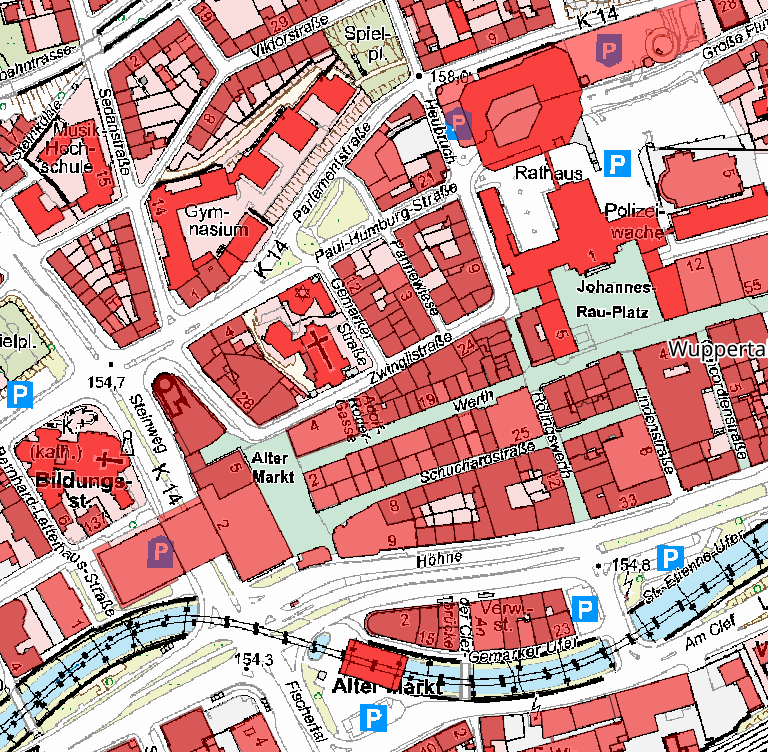
\includegraphics[width=0.3\textwidth]{Medien/own/hu_vergleich/qgis_hu_vergleich_abk_lanuv.png}
				\label{fig:analyse:hu_vergleich_detail_08}}
			\subfloat[Subfigure 9 list of figures text][ABK + OSM]{
				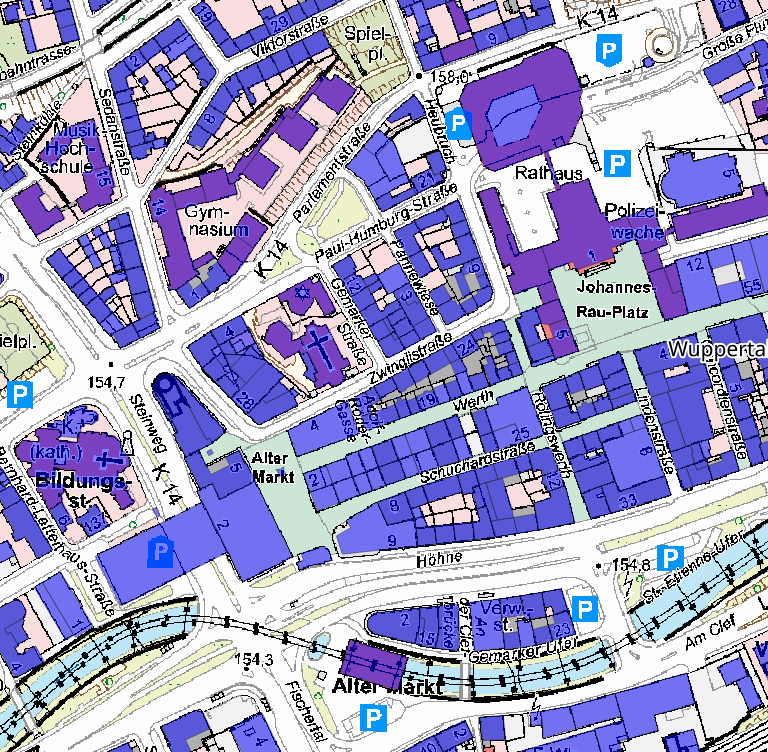
\includegraphics[width=0.3\textwidth]{Medien/own/hu_vergleich/qgis_hu_vergleich_abk_osm.png}
				\label{fig:analyse:hu_vergleich_detail_09}}
			\qquad
			\subfloat[Subfigure 10 list of figures text][ALKIS + LANUV]{
				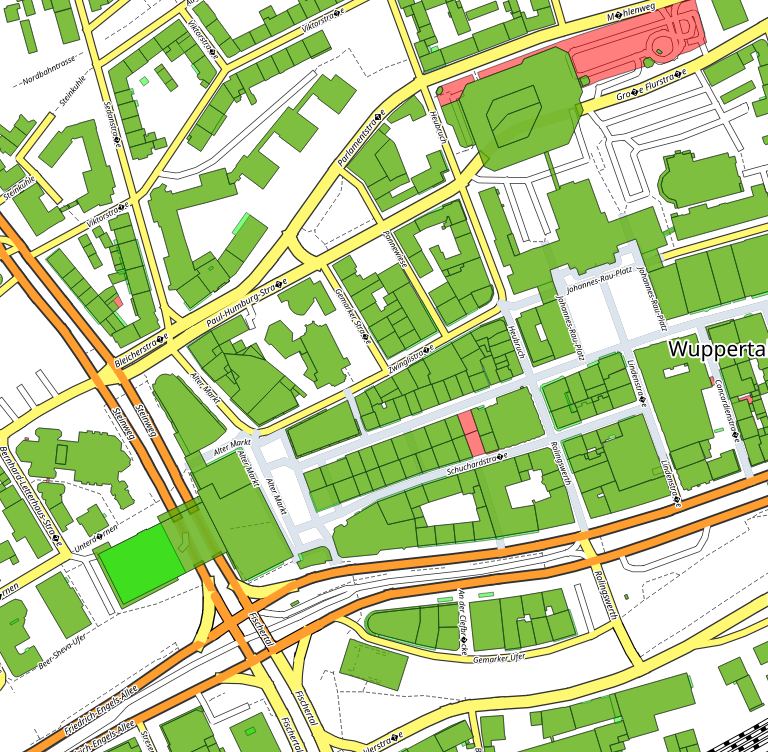
\includegraphics[width=0.3\textwidth]{Medien/own/hu_vergleich/qgis_hu_vergleich_alkis_lanuv.png}
				\label{fig:analyse:hu_vergleich_detail_10}}
			\subfloat[Subfigure 11 list of figures text][ALKIS + OSM]{
				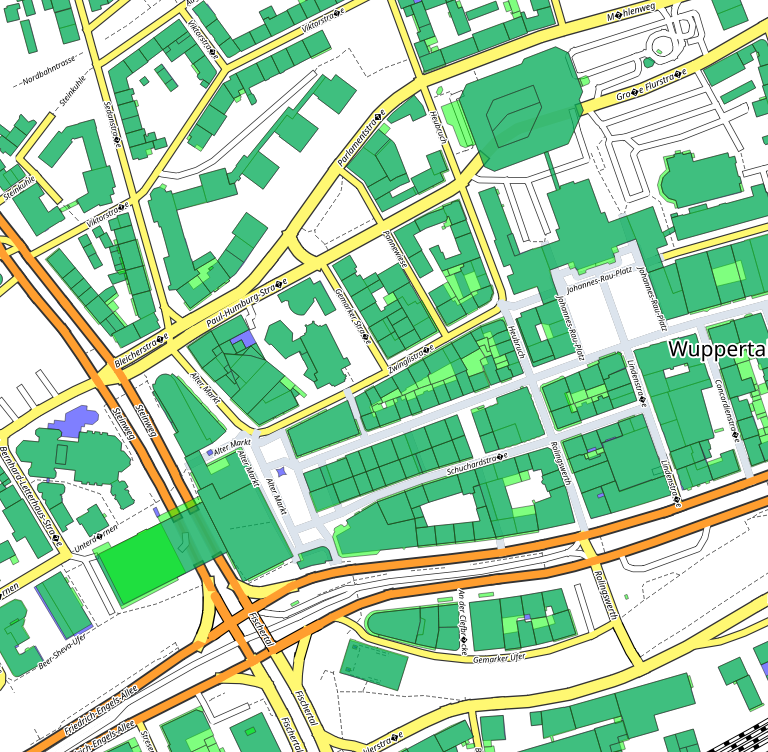
\includegraphics[width=0.3\textwidth]{Medien/own/hu_vergleich/qgis_hu_vergleich_alkis_osm.png}
				\label{fig:analyse:hu_vergleich_detail_11}}
			\subfloat[Subfigure 12 list of figures text][OSM + LANUV]{
				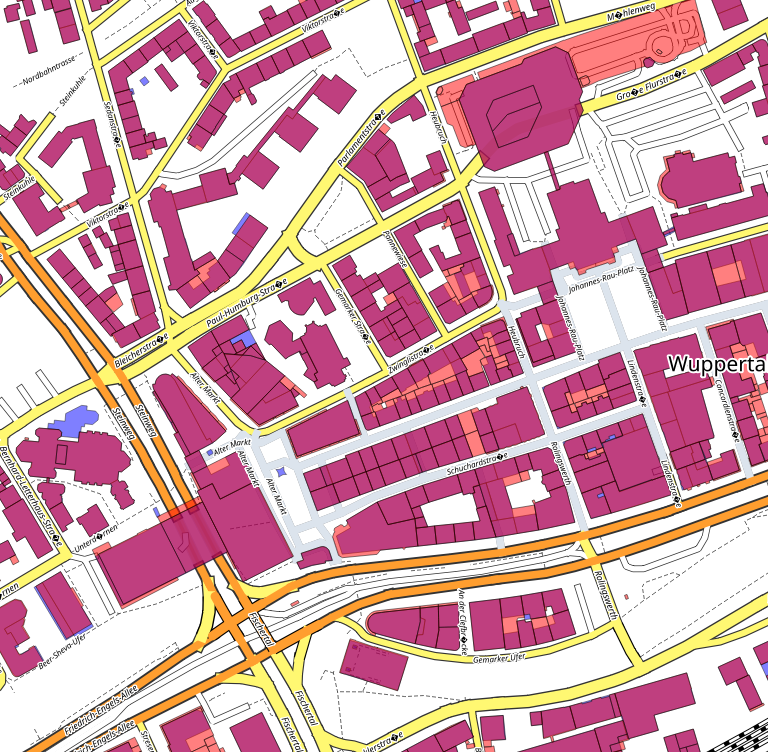
\includegraphics[width=0.3\textwidth]{Medien/own/hu_vergleich/qgis_hu_vergleich_lanuv_osm.png}
				\label{fig:analyse:hu_vergleich_detail_12}}
			\caption{Vergleich der Hausumringe-Geometrie in den Datensätzen (ALKIS, LANUV, OSM), Detailansicht}
			\label{fig:analyse:hu_vergleich_detail}
		\end{figure}

	
	